\chapter{Numerical simulations of restricted diffusion}
\label{ch:comp_res}\lettrine[lines=2, lhang=0.33, loversize=0.25]{I}{
n general, the diffusion coefficient} of a smaller molecule is reduced less during the
transition from solution to the cytosol than the \ac{DC} of a larger
molecule \cite{Shorten_09_BiophysJ_96_p4764}. For example, if we consider
the diffusion restrictions imposed by actomyosin, then the larger
molecule, such as \DEX, would not be able to pass through some of the
openings in the spatial structure which are traversable to smaller molecules such as \ATP.
This would results, predictably, in the \ac{DC} of \DEX\ being reduced
more in the cytosol than \ATP. However, as can seen from our experimental
results from \ref{ch:exp_res}, the \ac{DC} of the smaller molecule is reduced more in
transition from solution to \ac{CM} cytosol compared to the larger molecule. 
As shown by earlier modelling studies of respiration kinetics, diffusion
in \acp{CM} could be restricted by local barriers
\cite{Vendelin_04_MolCellBiochem_256_p229,Ramay_09_BiophysJ_97_p443}.
We explored this possibility be testing whether simple planar
permeable barriers could restrict diffusion of fluorescent dyes to the extend established from experiments shown in \ref{ch:exp_res}. 

\section{Computational model setup}
A stochastic computational model of diffusion was used to perform
\ac{RICS} experiments \insilico.

\begin{figure}[b!]
  \centering
%    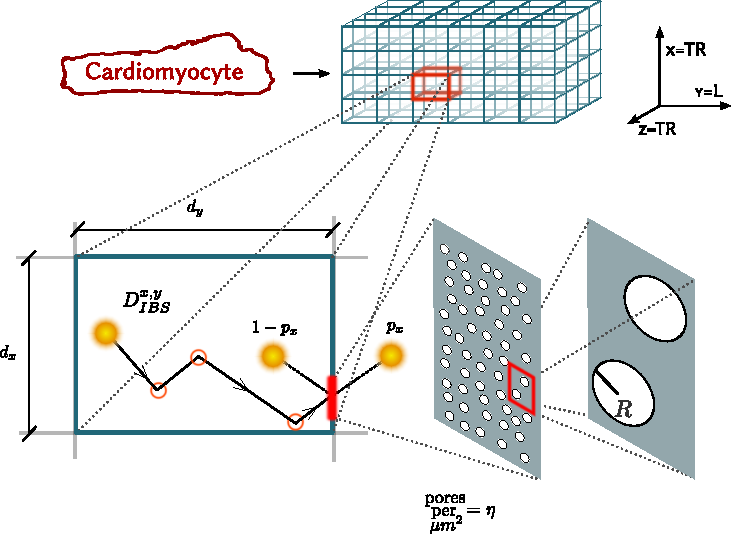
\includegraphics[width=10cm]{figures/model.pdf}
    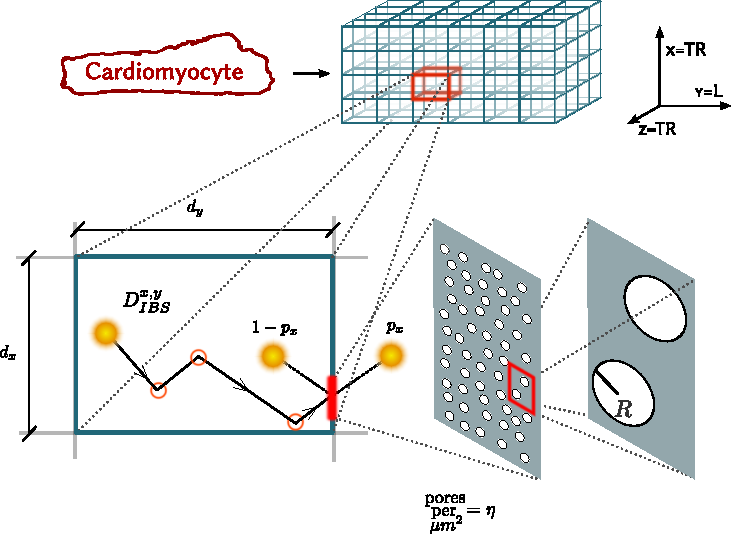
\includegraphics[width=10cm]{figures/model.pdf}
    \caption[Computational model scheme]{Scheme of the computational model. Intracellular
    structure of the cell (top left) is approximated by a 3D lattice of
    barriers which hinder molecule diffusion (top right). Barriers are
    placed, depending on direction $\alpha$, $d_\alpha$ $\mu$m apart and
    have permeabilities $p_\alpha$. Diffusion coefficient in the space
    between barriers is reduced by a factor $\lambda$ compared to
    solution ($0<\lambda\le1$). Stochastically diffusing molecules
    interact with barriers and have a probability $p_\alpha$ of passing
    through (bottom left). Permeable barriers correspond to porous
    walls with $\eta$ pores of radius $R$ per $\mu$m$^2$ of barrier area
    (bottom right). Apparent diffusion coefficients are estimated over
    the entire lattice by employing \ac{RICS} analysis on images
    acquired from the model.}
  \label{fig:model_scheme}
%The autocorrelation at shift vector $\Delta \mathbf{h}=(\xi,\psi)$ for an image with
%fluorescence values $F(\mathbf{p})$ at location $\mathbf{p} = (x,y)$ is given by:
%{\small
\end{figure}
Full details of the mathematical model are presented in \PaperIII. In
short, the model consisted of a lattice of permeable barriers 
separated from each other by a certain distance (as depicted on
\F{\ref{fig:model_scheme}}). Fluorescent dye
molecules diffuse in the \ac{IBS} with a \ac{DC} that
is reduced compared to the \ac{DC} in solution by a factor $\lambda$
(i.e., $DC_{IBS} = \lambda\cdot DC_{solution}$). Barrier permeability (resulting from $\eta$
pores of radius $R$ nm per $\mu$m$^2$ of barrier area) and
barrier-to-barrier distance ($d$), as well as the reduction of the \ac{DC} in the
inter barrier space ($\lambda$) were parameters which were estimated with the aid of
the computational model. Parameters were allowed to be
different in different spatial directions (longitudinal - L and
transverse - TR). 
\begin{figure}[t!]
  \centering
    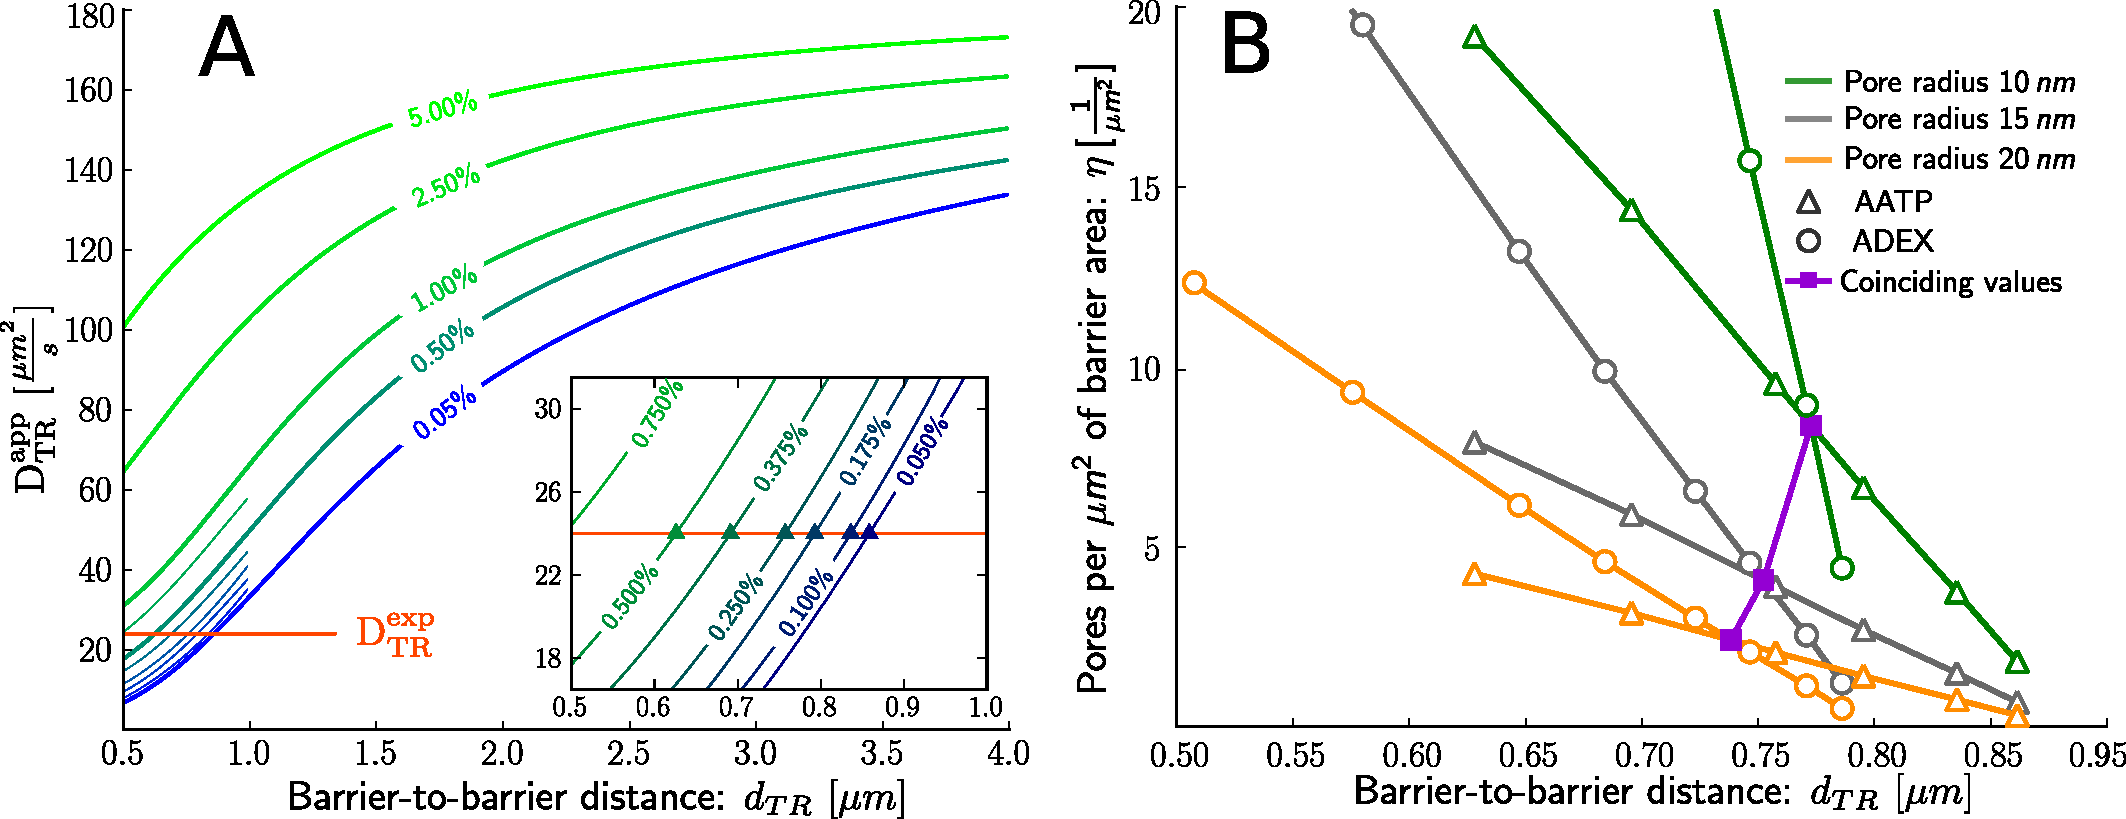
\includegraphics[width=12cm]{figures/mode_res.pdf}
    \caption[Computational model results]{(A) Apparent diffusion constant values for \ATP\
    are obtained from simulations with varying barrier distances
    (horizontal axis) and permeabilities (indicated by values on
    curves). Horizontal solid line shows \ATP\ diffusion
    coefficient estimated from experiment ($D^{exp}_{TR}$). Inset covers
    the region $0.5\ldots 1 \,\mu$m where curves intersect with
    experimental data. Intersection points are marked with triangles.
    (B) Points of intersection from A with permeability converted to
    pores per $\mu$m$^2$ for different pore radius
    values (10, 15 and 20 nm). Intersections of \ATP\ ($\triangle$) and
    \DEX\  (\protect \raisebox{-1pt}{\Large $\circ$}) curves of
    identical pore radius values signify points where model and
    experiment coincide for both molecules
    simultaneously($\blacksquare$). Intersections are curves in 3D space
    (barrier-to-barrier distance vs. pore radius vs. pores per {\small
    $\mu$}m$^2$).}
  \label{fig:model_res}
%The autocorrelation at shift vector $\Delta \mathbf{h}=(\xi,\psi)$ for an image with
%fluorescence values $F(\mathbf{p})$ at location $\mathbf{p} = (x,y)$ is given by:
%{\small
\end{figure}

Together with simulating stochastic diffusion, the model generated
images similar to those obtained from confocal microscopy experiments.
\ac{RICS} analysis was applied to these images and apparent \acp{DC}
estimated. The apparent \ac{DC} determined by \ac{RICS} is the result
of molecules diffusing in the inter-barrier space and interacting with
the permeable barriers. A collection of apparent \ATP\ \acp{DC} obtained from
modelling are presented in \F{\ref{fig:model_res}}A. The dependence of 
the apparent \ac{DC} estimated from the model is plotted as a function 
of barrier-to-barrier distance for various barrier permeability values. 
It can be seen that as barrier permeability increases, the effect of the
barriers on the apparent \ac{DC} decreases. Since the actual \ac{DC} was
estimated from experiments on cardiomyocytes as presented in
\ref{ch:exp_res}, it is possible to find at which barrier-to-barrier
distance and barrier permeability values the model produces the same
apparent \ac{DC} as the experiment. It is helpful to explain the
procedure in terms of intersections on plots in parameter space. For this, the experimentally estimated \ac{DC} is
plotted on the graph of model results (the horizontal line
$D_\mathrm{TR}^{exp}$ in \F{\ref{fig:model_res}}A). At points where
model result curves and the line representing the experimental
value intersect, the model yields the experimentally obtained \ac{DC}.
For clarity the intersection region is magnified in the inset of 
\F{\ref{fig:model_res}}A. The same procedure is performed for \DEX\ with
the experimentally determined \ac{DC} of \DEX\ in \ac{CM} used for finding
intersections. 

As a result of this we obtain a set of barrier-to-barrier, permeability
value pairs for both \ATP\ and \DEX\ at which the computational model of
restricted diffusion yields experimentally obtained \acp{DC}. As
explained in \PaperIII, barrier permeability values for \ATP\ and \DEX\
are not directly comparable. It is possible, however, to convert from barrier
permeability to the number of pores per unit barrier area ($\eta$) by fixing a
certain pore radius (R). These two parameters are independent of the
diffusing dye, allowing the model parameter values obtained for \ATP\ and \DEX\ to be
compared. This is done by plotting them together for different pore
radius values (\F{\ref{fig:model_res}}B). At points where \ATP\ and
\DEX\ curves intersect, the computational model is able to reproduce the
experimentally estimated \acp{DC} for both \ATP\ and \DEX\
simultaneously. From \F{\ref{fig:model_res}}B it is possible
to establish the range of parameters (d, $\eta$, R) at which the model
is able to match results from experiments on cardiomyocytes. 

\section{Barrier properties estimated from computational model}

The ranges collected from intersections in \F{\ref{fig:model_res}}B
represent parameter values where both \ATP\ and \DEX\ are able to simultaneously
match experimental \acp{DC} and are presented as the results from the
computational  model in Table \ref{table:model_res}. In general,
barriers need to be spaced $\sim$ 1 $\mu$m from each other, have a small
number of nanometer scale pores, and the \ac{DC} in the inter-barrier
should be comparable to \ac{DC} in solution in order for the model to
reproduce experimental results.
\begin{table}
\begin{center}
\begin{tabular}{lcccc}

  \hline
  & \multicolumn{4}{c}{Direction} \\
  Model & \multicolumn{2}{c}{transverse} &
  \multicolumn{2}{c}{longitudinal} \\ 
  parameter& \multicolumn{2}{c}{TR (x,z)} & \multicolumn{2}{c}{L (y)} \\
  &min&max&min&max\\
  \hline
  Distance d [$\mu$m] & $0.68\pm 0.10$ & $0.87\pm 0.07$ &
  $0.73\pm 0.13$&$1.02\pm 0.10$ \\
  Pore radius R [nm]  & $7.4 \pm 2.1$ & $30 \pm 8$&
  $6.7\pm 1.8 $&$38\pm 10$\\
  Pore density $\eta$ [$\sfrac{1}{\mu \mathrm{m}^2}$] & $1.2 \pm 0.1$ &
  $29 \pm 23$ & $1.1\pm 0.1$ & $48\pm37$ \\
  $\lambda^{\mathrm{AATP}}$ & $0.78 \pm 0.13$ & $1.0$&$0.78 \pm 0.13$ &$1.0$ \\
  $\lambda^{\mathrm{ADEX}}$ & $0.77 \pm 0.14$ & $1.0$&$0.77 \pm 0.14$ &$1.0$ 
\end{tabular}

\end{center}
\caption[Properties of barriers restricting diffusion]{Properties of
barriers restricting diffusion predicted by stochastic model on the
basis of RICS measurements. Data presented is mean$\pm$standard
deviation.}
\label{table:model_res}
\end{table}

Errors for the model parameters were estimated by Monte Carlo simulation
outlined in the Supporting Material of \PaperIII. Since the minimal and
maximal values of some of the parameters do not follow a normal
distribution, the mean and standard deviation values are less
informative than the shape of the actual distribution for which the Supporting Material of \PaperIII
should be consulted. 
%\section{Diffusion obstacle parameter sensitivity}
%
%Parameters presented in Table 2 of the main text were obtained by
%finding intersections between curves of experimental and computational
%results. As visible from Figures 2C,2D and 2E in the main text, a range
%of barrier-to-barrier distance, pore radius and pore density values
%satisfy the constraints of the model and computational results.
%The experimentally obtained \ac{DC}\ values have a error associated with
%them. In order to estimate the uncertainties caused by measurement errors
%in the parameters we found, Monte Carlo analysis was applied. Similar to the procedure
%depicted on Figure 2B and 2C, random \ac{DC}\ for \ATP\ and \DEX\ were
%chosen from a normal distribution with the mean and standard deviation
%equal to the values from experiments presented in Table 1 (i.e.,
%$\mathcal{N}(24,6)$, $\mathcal{N}(16,2)$ for \ATP\ and \DEX\ in the
%transverse direction and $\mathcal{N}(35,8)$, $\mathcal{N}(19,3)$ in the
%longitudinal direction). For each randomly generated \ATP\ \DEX\ \ac{DC}\  value pair,
%intersections were found and from those a range of suitable parameter
%values determined. Random sampling was performed 300000 times for both
%transverse and longitudinal  directions. The resulting distribution of
%random \ac{DC}\ value pairs are shown on \F{~\ref{fig:stats_d}A and B} for
%the transverse and longitudinal directions, respectively. Of possible
%combinations two types were discarded. First, cases where \ac{DC}\ of \DEX\
%was larger than \ATP\ (left of the dashed lines and on
%\F{~\ref{fig:stats_d}}) and, secondly, cases where the pore density value
%was so low that less than one would be present on a single barrier element
%(the middle, light region on \F{~\ref{fig:stats_d}}). For all other
%pairs model parameter maximum and minimum values were obtained and
%collected. Histograms for obtained maximum and
%minimum parameter values are presented in \Fs{~\ref{fig:stats_x} and
%\ref{fig:stats_y}}. Histograms for maximum estimate of \ac{DC}\ reduction
%values are not shown as they were always 100\% of the \ac{DC}\ in solution. 
%The results presented in Table 2 in the main text are the mean and standard
%deviations of these distributions.
%%In some cases intersections could not be obtained,
%%meaning that for those \ATP\ \DEX\ \ac{DC} value pairs there are no barrier
%%As \ac{DC}\ values closer to the mean experimental value were more likely to
%%occur the 
%\begin{figure*}[b]
%  \centering
%  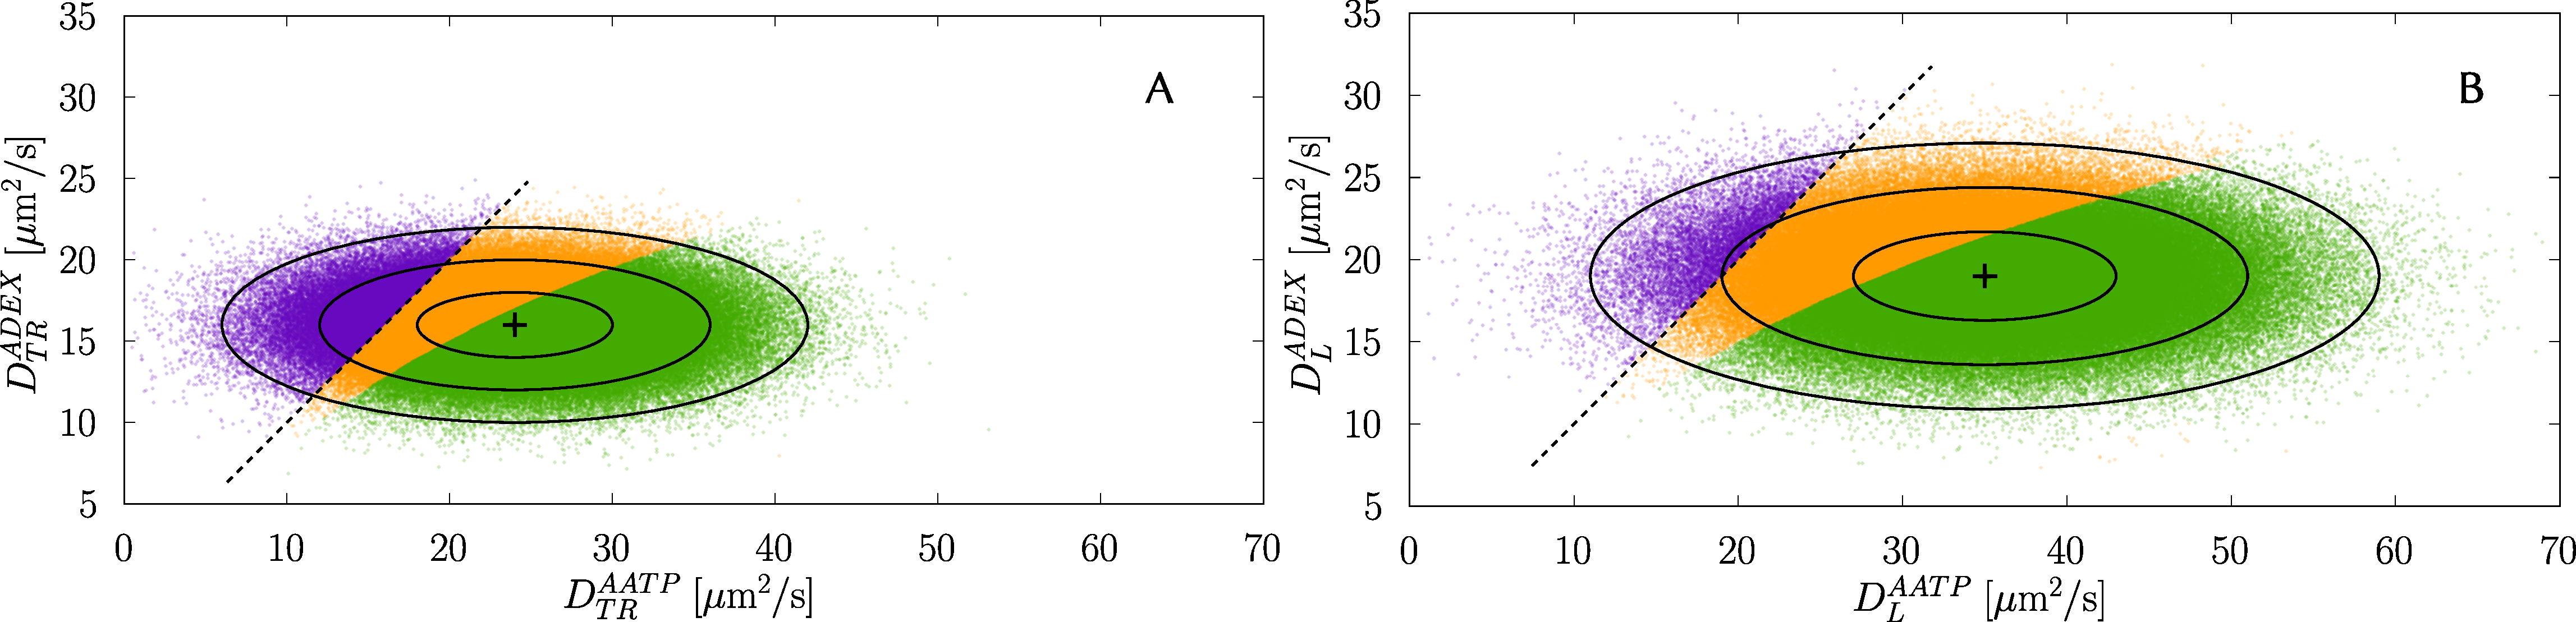
\includegraphics[width=12cm]{figures/stat_d.pdf}
%  \caption[short]{ Distributions of random generated pairs of \ATP\ and \DEX\ diffusion
%  coefficients in transverse(A) and longitudinal directions (300000
%  values each). Pairs were
%  randomly generated from normal distributions having the mean and
%  standard deviation obtained from experiment (shown in Table 1 of
%  the main text. Experimental mean values are shown with a cross.
%  Ellipses indicate distances 1,2 and 3 standard deviations from the mean. Dotted
%  line show \ac{DC}\ values of \ATP\ and \DEX\ are equal. As explained in
%  the text, values left of this line are discarded and not included in analysis. The middle
%  region(shown in yellow) contains \ac{DC}\ value pairs where density of
%  pores in barrier would be less then 1 per barrier. For the \ac{DC}\ values in the green region
%  intersections are found as in the main text and collected for
%  statistics. }
%  \label{fig:stats_d}
%\end{figure*}
%
%\begin{figure*}[t]
%      \centering
%      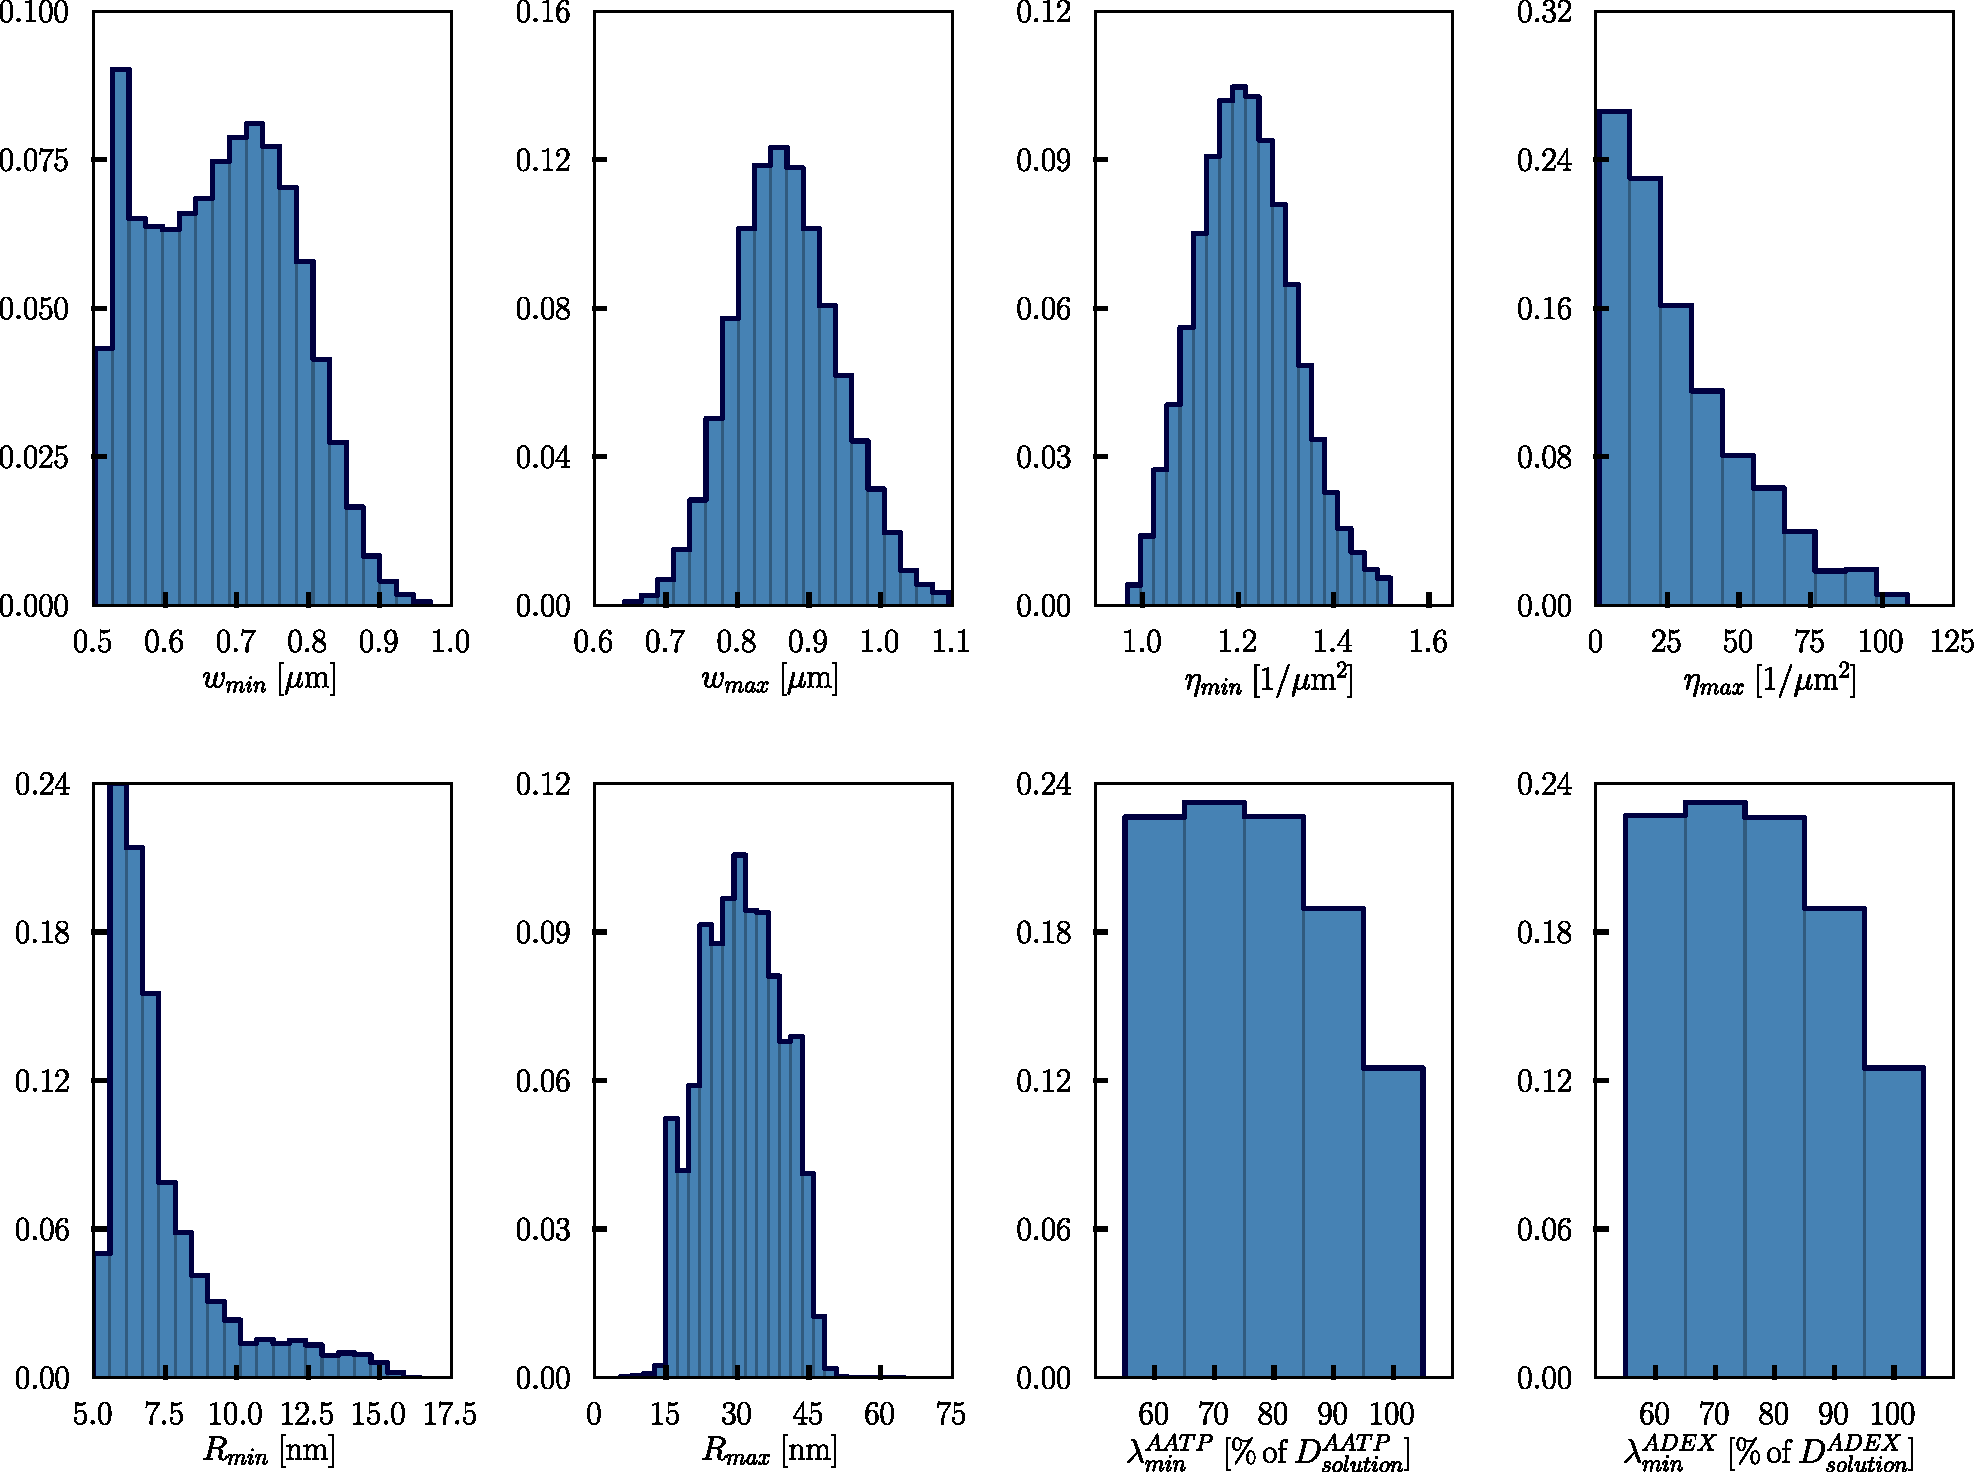
\includegraphics[width=12cm]{figures/stat_x_h.pdf}
%      \caption[short]{ Histograms showing distributions of minimum and maximum model parameter
%      values obtained from Monte Carlo simulations in the transverse
%      direction. }
% \label{fig:stats_x}
%\end{figure*}
%
%\begin{figure*}
%      \centering
%      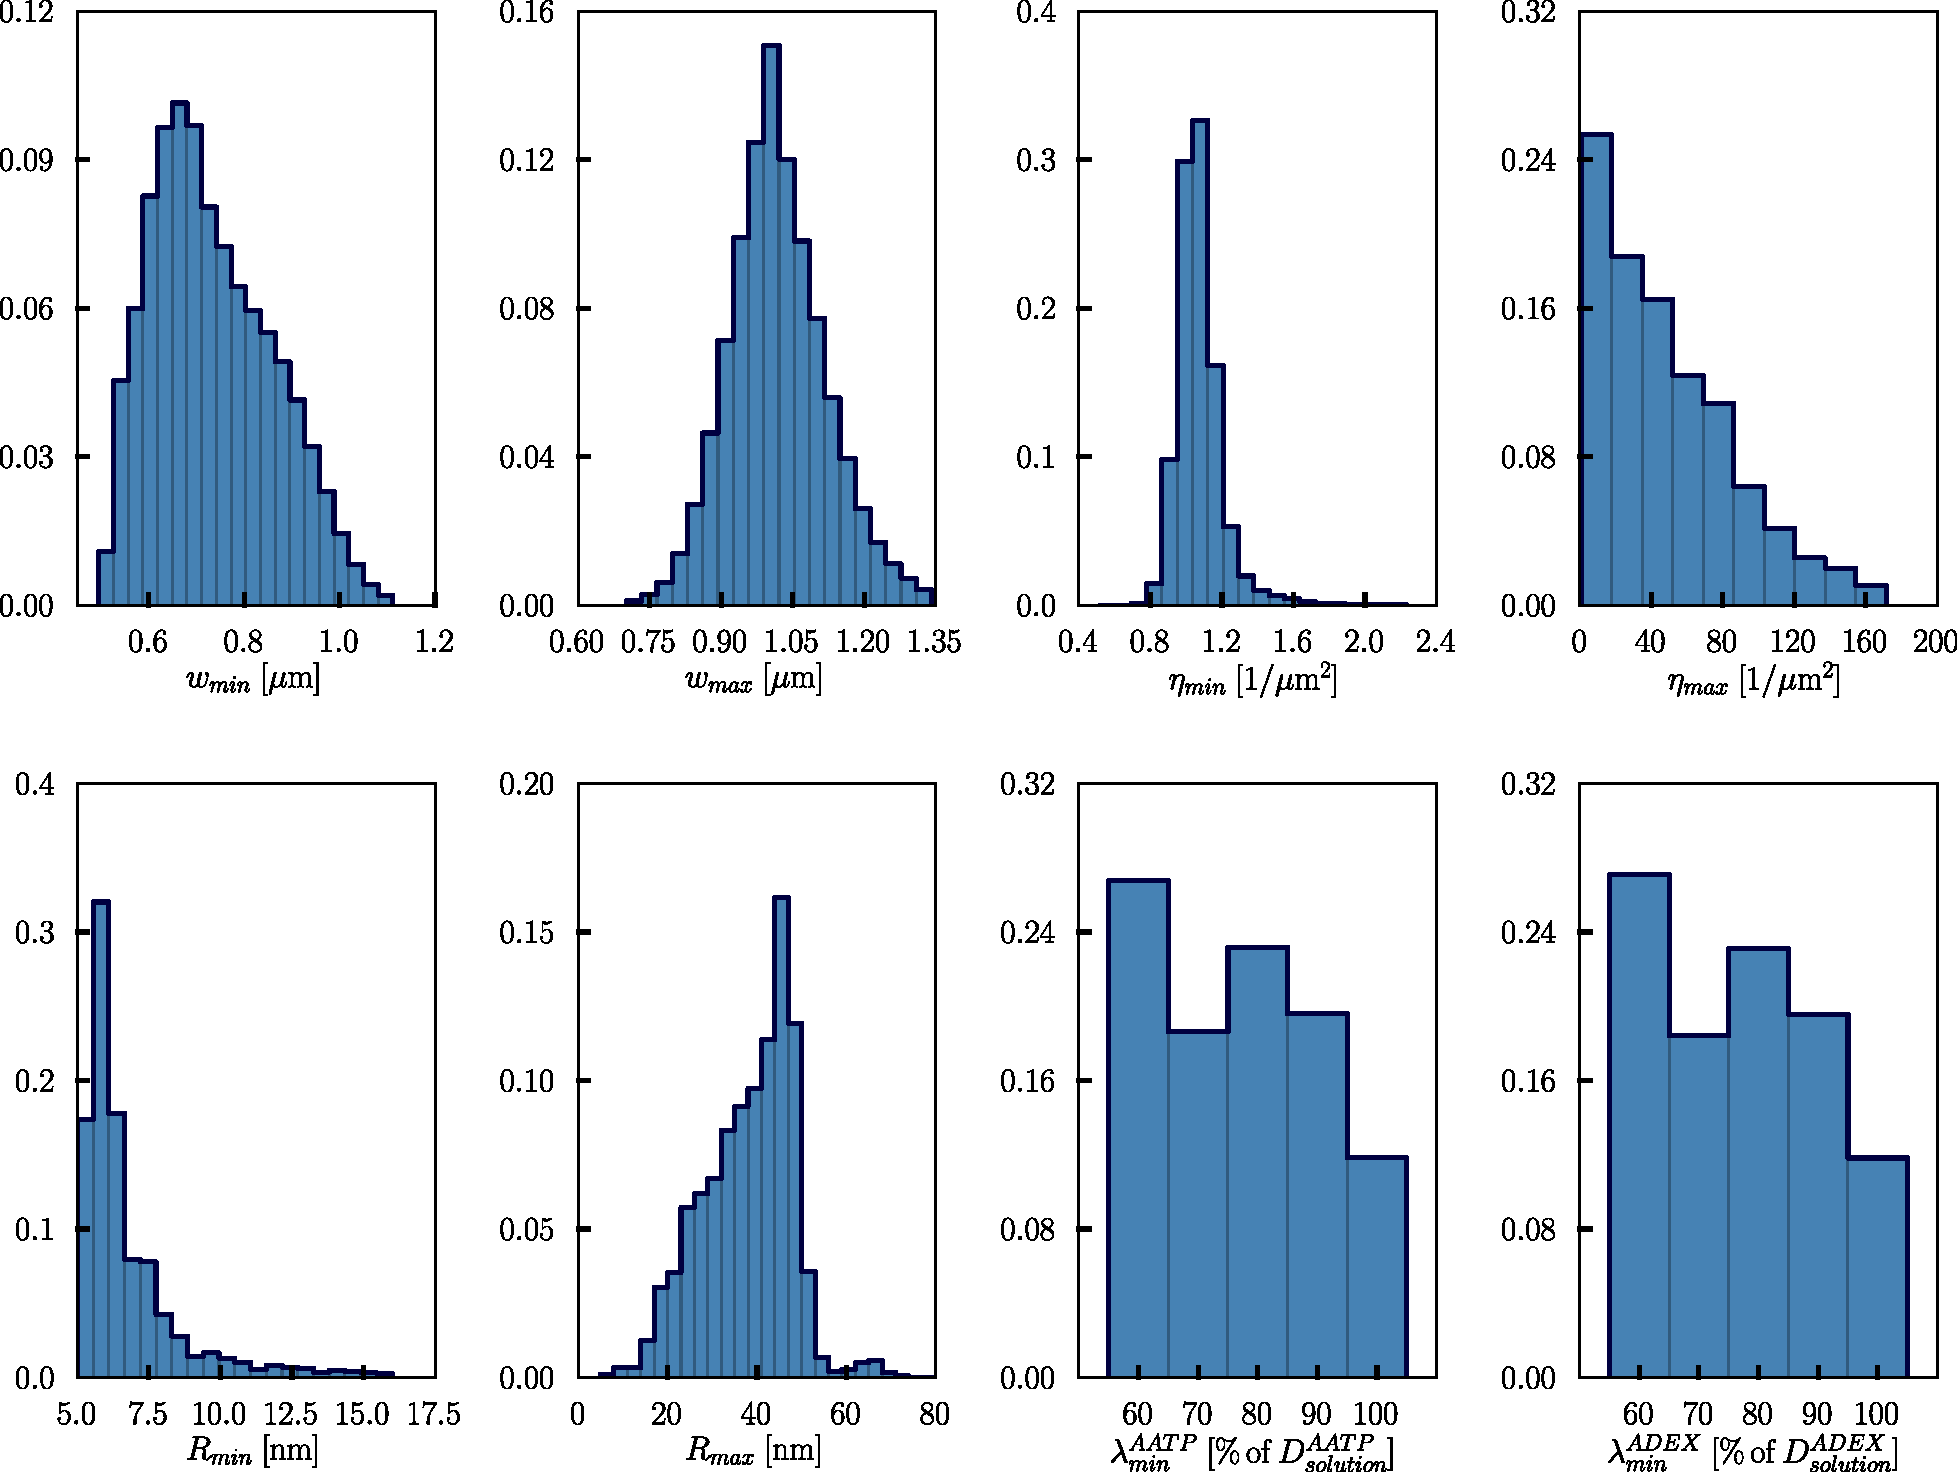
\includegraphics[width=12cm]{figures/stat_y_h.pdf}
%      \caption[short]{ Histograms showing distributions of minimum and maximum model parameter
%      values obtained from Monte Carlo simulations in the longitudinal
%      direction. }
% \label{fig:stats_y}
%\end{figure*}

\section{Conclusions}
The stochastic model for simulating restricted diffusion with regular permeable
barriers can match  experimentally found \acp{DC} for
\ATP\ and \DEX\ in the case when: 

\begin{itemize}
  \item barriers in the model are located relatively close to each other ($<$1 $\mu$m apart)
  \item permeability of these barriers is relatively low (containing
$\sim$ 1$\ldots$40 pores of radius 7$\ldots$30 nm per $\mu$m$^2$)
    \item the \ac{DC} in the inter-barrier space is lower than that of diffusion
in solution by a factor 0.8$\ldots$1. 
\end{itemize}
Diffusional anisotropy results in
the ranges of the parameters differing slightly in different spatial
directions as visible from Table \ref{table:model_res}.

The choice of model geometry employed here, whereby regularly placed
semi-permeable barriers cause restrictions to diffusion, is not the only
geometry that can explain the paradoxical result where a smaller
molecule is restricted more than a larger one. Our model setup was
motivated by its relative simplicity compared to more complex
geometries. Although already this simple geometry
was able to give an answer to the raised question, more complicated
model geometries with sub-volumes excluding the larger dye could be
explored in the future.
